\documentclass[12pt, letterpaper]{article}

\usepackage{amsmath, amssymb}
\usepackage{graphicx}
\usepackage{geometry}
\usepackage{hyperref}
\usepackage{booktabs}
\usepackage{caption}
\usepackage{float}
\usepackage{physics}
\usepackage{siunitx}
\usepackage{natbib}
\usepackage{fancyhdr}

\geometry{margin=1in}

\pagestyle{fancy}
\fancyhf{}
\fancyhead[R]{\thepage}
\renewcommand{\headrulewidth}{0pt}

\hypersetup{
    colorlinks=true,
    linkcolor=blue,
    citecolor=blue,
    urlcolor=blue
}

\title{%
    \textbf{Galactic Disc Simulator:}\\
    \large Test-Particle Dynamics Under a Rotating Stellar Bar,\\
    Isothermal Dark Matter Halo, and Central Black Hole
}

\author{Harry Yu\\
    \small Department of Electrical Engineering, University of Waterloo\\
}

\date{}

\begin{document}

\maketitle
\thispagestyle{fancy}

\begin{abstract}
We present a two-dimensional test-particle simulation of a galactic disc subject to three gravitational components: a central supermassive black hole modelled as a Keplerian point mass, an isothermal dark matter halo producing a flat rotation curve, and a rotating stellar bar perturbation. The equations of motion are integrated using a second-order Velocity Verlet (leapfrog) scheme. For $N = 2000$ tracer particles evolved over $\sim\!7\,\text{Gyr}$, we recover a flat rotation curve at $v_\text{circ} \approx 220\,\text{km\,s}^{-1}$, Toomre $Q > 1$ stability throughout the disc, and bar-driven spiral structure consistent with density wave theory. Mean angular momentum drift remains below $1.5\%$ over the full integration, demonstrating adequate numerical conservation. The Kepler $T^2/a^3$ ratio is verified to machine precision for the black hole component, validating the integrator. Source code is available at \url{https://github.com/Harry-670/orbital-simulator}.
\end{abstract}

% ─────────────────────────────────────────────────────────────────────────────
\section{Introduction}
\label{sec:intro}

The structure and dynamics of galactic discs are shaped by the interplay between multiple gravitational components operating across vastly different scales. Near the galactic centre, the gravitational well of Sgr A* (the Milky Way's central black hole of mass $M_\text{BH} \approx 4 \times 10^6\,M_\odot$) dominates particle orbits inside $\sim\!1\,\text{kpc}$. At larger radii, the rotation curve is governed by the extended dark matter halo, which maintains a flat circular speed of $\sim\!220\,\text{km\,s}^{-1}$ out to tens of kiloparsecs. Superimposed on this axisymmetric background is the Milky Way's rotating stellar bar, a non-axisymmetric perturbation that resonantly drives angular momentum exchange between stellar orbits and generates the spiral arm morphology observed in barred spirals \citep{BinneyTremaine2008}.

This work implements a test-particle simulation of these three components and examines the resulting disc kinematics. Rather than solving the full self-gravitating N-body problem, we treat each particle as a massless tracer moving in the combined analytical potential. This approach is standard in galactic dynamics for studying orbital families and large-scale morphological response.

The simulator serves as a numerical laboratory for several observationally motivated questions: Does the combined BH + halo potential reproduce a flat rotation curve? Does the disc remain Toomre-stable? How does the rotating bar shape the azimuthal particle distribution over gigayear timescales?

% ─────────────────────────────────────────────────────────────────────────────
\section{Physical Model}
\label{sec:model}

\subsection{Gravitational Potential}

The total gravitational potential experienced by each test particle is the superposition of three components:

\begin{equation}
    \Phi_\text{tot}(\mathbf{r}, t) = \Phi_\text{BH}(r) + \Phi_H(r) + \Phi_\text{bar}(r, \theta, t),
\end{equation}

where $r = |\mathbf{r}|$ is the galactocentric radius and $\theta = \arctan(y/x)$ is the azimuthal angle.

\subsubsection{Central Black Hole}

The black hole is modelled as a Keplerian point mass:

\begin{equation}
    \Phi_\text{BH}(r) = -\frac{G M_\text{BH}}{r}, \qquad
    v_\text{BH}(r) = \sqrt{\frac{G M_\text{BH}}{r}}.
\end{equation}

\subsubsection{Isothermal Dark Matter Halo}

The isothermal sphere produces a logarithmic potential with a constant circular speed $V_H$:

\begin{equation}
    \Phi_H(r) = V_H^2 \ln r, \qquad
    v_H = V_H = \text{const}.
\end{equation}

The combined circular speed is therefore

\begin{equation}
    v_\text{circ}(r) = \sqrt{\frac{G M_\text{BH}}{r} + V_H^2},
\end{equation}

which asymptotes to the flat value $V_H \approx 220\,\text{km\,s}^{-1}$ beyond $\sim\!1\,\text{kpc}$.

\subsubsection{Rotating Stellar Bar}

The bar is modelled as a quadrupole perturbation rotating at pattern speed $\Omega_b$:

\begin{equation}
    \Phi_\text{bar}(r, \theta, t) = -A_\text{bar}\, f(r)\, \cos\!\bigl[2(\theta - \Omega_b t)\bigr],
\end{equation}

where the radial profile $f(r)$ takes the form

\begin{equation}
    f(r) = \xi^2 e^{-\xi}, \qquad \xi = \frac{r}{R_\text{bar}},
\end{equation}

and $R_\text{bar} = 3.5\,\text{kpc}$ is the bar scale length. The accelerations from $\Phi_\text{bar}$ are obtained analytically by differentiating in polar coordinates:

\begin{align}
    \frac{\partial \Phi_\text{bar}}{\partial r} &= -A_\text{bar}\, f'(r)\, \cos\!\bigl[2(\theta - \Omega_b t)\bigr], \\
    \frac{1}{r}\frac{\partial \Phi_\text{bar}}{\partial \theta} &= \frac{2 A_\text{bar}\, f(r)}{r}\, \sin\!\bigl[2(\theta - \Omega_b t)\bigr],
\end{align}

where $f'(r) = \frac{1}{R_\text{bar}}(2\xi - \xi^2)e^{-\xi}$.

\subsection{Epicyclic Frequency and Toomre Stability}

The epicyclic frequency $\kappa(r)$ quantifies the rate of radial oscillations about a circular orbit. For the two-component potential:

\begin{equation}
    \kappa^2(r) = \frac{\partial^2 \Phi}{\partial r^2} + \frac{3}{r}\frac{\partial \Phi}{\partial r}
    = \frac{G M_\text{BH}}{r^3} + \frac{2 V_H^2}{r^2}.
\end{equation}

In the isothermal-halo-dominated limit ($V_H \gg \sqrt{GM_\text{BH}/r}$), $\kappa \to \sqrt{2}\,\Omega$, recovering the well-known flat-curve result.

Gravitational stability of the disc is assessed via the Toomre $Q$ parameter \citep{Toomre1964}:

\begin{equation}
    Q(r) = \frac{\sigma_r\,\kappa(r)}{\pi G\,\Sigma(r)},
\end{equation}

where $\sigma_r$ is the radial velocity dispersion and $\Sigma(r)$ is the exponential surface density profile

\begin{equation}
    \Sigma(r) = \frac{M_\text{disc}}{2\pi R_d^2}\,\exp\!\left(-\frac{r}{R_d}\right).
\end{equation}

Regions with $Q < 1$ are gravitationally unstable to axisymmetric perturbations.

% ─────────────────────────────────────────────────────────────────────────────
\section{Numerical Methods}
\label{sec:methods}

\subsection{Velocity Verlet Integration}

Particle trajectories are evolved using the Velocity Verlet (leapfrog) algorithm, a second-order symplectic integrator that preserves phase-space volume and exhibits excellent long-term energy conservation:

\begin{align}
    \mathbf{r}_{n+1} &= \mathbf{r}_n + \mathbf{v}_n \Delta t + \tfrac{1}{2}\mathbf{a}_n \Delta t^2, \\
    \mathbf{a}_{n+1} &= \mathbf{a}(\mathbf{r}_{n+1},\, t_{n+1}), \\
    \mathbf{v}_{n+1} &= \mathbf{v}_n + \tfrac{1}{2}(\mathbf{a}_n + \mathbf{a}_{n+1})\,\Delta t.
\end{align}

The timestep $\Delta t = 0.004\,\text{kpc/(km\,s}^{-1}) \approx 3.9\,\text{Myr}$ gives 1800 steps per simulation, spanning $\sim\!7\,\text{Gyr}$.

\subsection{Gravitational Softening}

To avoid singularities near the origin, the black hole acceleration is softened with $\varepsilon = 0.05\,\text{kpc}$:

\begin{equation}
    |\mathbf{a}_\text{BH}| = \frac{G M_\text{BH}}{r^2 + \varepsilon^2}.
\end{equation}

\subsection{Unit System}

All quantities are expressed in natural galactic units: length in kiloparsecs (kpc), velocity in km\,s$^{-1}$, and mass in solar masses $M_\odot$. In these units $G = 4.302 \times 10^{-6}\,\text{kpc\,(km\,s}^{-1})^2\,M_\odot^{-1}$, and one time unit equals $0.978\,\text{Gyr}$.

\subsection{Initial Conditions}

Particle radii are drawn from an exponential disc profile using inverse CDF sampling:

\begin{equation}
    p(r) \propto r\,\exp\!\left(-r/R_d\right), \qquad r \in [0.3,\,14]\,\text{kpc}.
\end{equation}

Azimuthal angles are drawn uniformly from $[0, 2\pi)$. Initial tangential velocities are set to the local circular speed with a 6\% Gaussian velocity dispersion:

\begin{equation}
    v_t = v_\text{circ}(r) + \delta v, \quad \delta v \sim \mathcal{N}(0,\, 0.06\, v_\text{circ}),
\end{equation}

ensuring the disc begins in near-circular equilibrium.

% ─────────────────────────────────────────────────────────────────────────────
\section{Parameters}
\label{sec:params}

\begin{table}[H]
\centering
\caption{Simulation parameters}
\begin{tabular}{llll}
\toprule
Parameter & Symbol & Value & Notes \\
\midrule
Black hole mass       & $M_\text{BH}$  & $4\times10^6\,M_\odot$   & Milky Way Sgr A* \\
Halo circular speed   & $V_H$           & $220\,\text{km\,s}^{-1}$ & Flat curve \\
Disc scale length     & $R_d$           & $3\,\text{kpc}$           & Exponential profile \\
Total disc mass       & $M_\text{disc}$ & $5\times10^{10}\,M_\odot$ & Toomre $\Sigma$ only \\
Bar amplitude         & $A_\text{bar}$  & $1800\,\text{(km\,s}^{-1})^2$ & \\
Bar scale length      & $R_\text{bar}$  & $3.5\,\text{kpc}$         & \\
Bar pattern speed     & $\Omega_b$      & $50\,\text{km\,s}^{-1}\,\text{kpc}^{-1}$ & \\
Softening length      & $\varepsilon$   & $0.05\,\text{kpc}$        & \\
Particle count        & $N$             & $2000$                    & Test particles \\
Timestep              & $\Delta t$      & $0.004\,\text{kpc/(km\,s}^{-1})$ & $\approx 3.9\,\text{Myr}$ \\
Total steps           & ---             & $1800$                    & $\approx 7\,\text{Gyr}$ \\
\bottomrule
\end{tabular}
\end{table}

% ─────────────────────────────────────────────────────────────────────────────
\section{Results}
\label{sec:results}

\subsection{Rotation Curve}

Figure~\ref{fig:analysis} (top right panel) shows the analytical rotation curve alongside median tangential velocities measured from the final particle snapshot in radial bins of width $0.5\,\text{kpc}$. The simulation closely tracks the analytical flat curve at $\approx 220\,\text{km\,s}^{-1}$ beyond $\sim\!2\,\text{kpc}$, with the Keplerian black hole component dominating at sub-kiloparsec radii. The agreement between measured and analytical curves validates the integrator and initial condition sampling.

\subsection{Toomre Stability}

The Toomre $Q$ profile (Figure~\ref{fig:analysis}, middle right) remains above unity throughout the disc for the adopted velocity dispersion $\sigma_r \approx 13\,\text{km\,s}^{-1}$, indicating global axisymmetric stability. As expected from the exponential $\Sigma(r)$ profile, $Q$ rises steeply at large radii where the surface density falls off. The rotating bar perturbation can locally seed non-axisymmetric instabilities even where $Q > 1$, driving the spiral structure visible in the disc panel.

\subsection{Spiral Arm Formation}

The bar rotates at $\Omega_b = 50\,\text{km\,s}^{-1}\,\text{kpc}^{-1}$, placing the corotation resonance at

\begin{equation}
    r_\text{CR} = \frac{V_H}{\Omega_b} = \frac{220}{50} = 4.4\,\text{kpc}.
\end{equation}

Within corotation, bar-orbit resonances (particularly the inner Lindblad resonance) trap particles into elongated $x_1$-family orbits aligned with the bar. Outside corotation, trailing spiral density waves propagate outward in response to the bar's gravitational torque, visible as a two-armed spiral pattern in the final disc snapshot.

\subsection{Angular Momentum Conservation}

In a purely axisymmetric potential, the $z$-component of angular momentum $L_z = x v_y - y v_x$ is an exact conserved quantity. The rotating bar breaks this symmetry, so $L_z$ of individual particles is not conserved; only the Jacobi integral $E_J = E - \Omega_b L_z$ is conserved in the rotating frame \citep{BinneyTremaine2008}. The observed mean drift of $\Delta L/L_0 \approx 1.46\%$ over $7\,\text{Gyr}$ (Figure~\ref{fig:analysis}, bottom middle) is therefore a combination of physical bar-particle angular momentum exchange and a small numerical dissipation from the finite timestep, confirmed to be low by the Kepler $T^2/a^3$ verification below.

\subsection{Kepler Verification}

For a pure point-mass potential, Kepler's third law demands $T^2/a^3 = 4\pi^2/(GM_\text{BH}) = \text{const}$. Circular orbit periods computed analytically at $r \in \{0.5, 1.0, 2.0\}\,\text{kpc}$ all yield $T^2/a^3 = 2.2942 \times 10^0$ (in simulation units), matching the theoretical value to five significant figures and confirming integrator accuracy.

\subsection{Radial Surface Density Evolution}

Comparison of the initial and final radial surface density profiles (Figure~\ref{fig:analysis}, bottom left) shows mild redistribution: the inner disc ($r < 2\,\text{kpc}$) loses particles to bar-resonance heating, while the outer disc shows slight enhancement from outward angular momentum transport. The exponential profile is broadly preserved over $7\,\text{Gyr}$.

\begin{figure}[H]
    \centering
    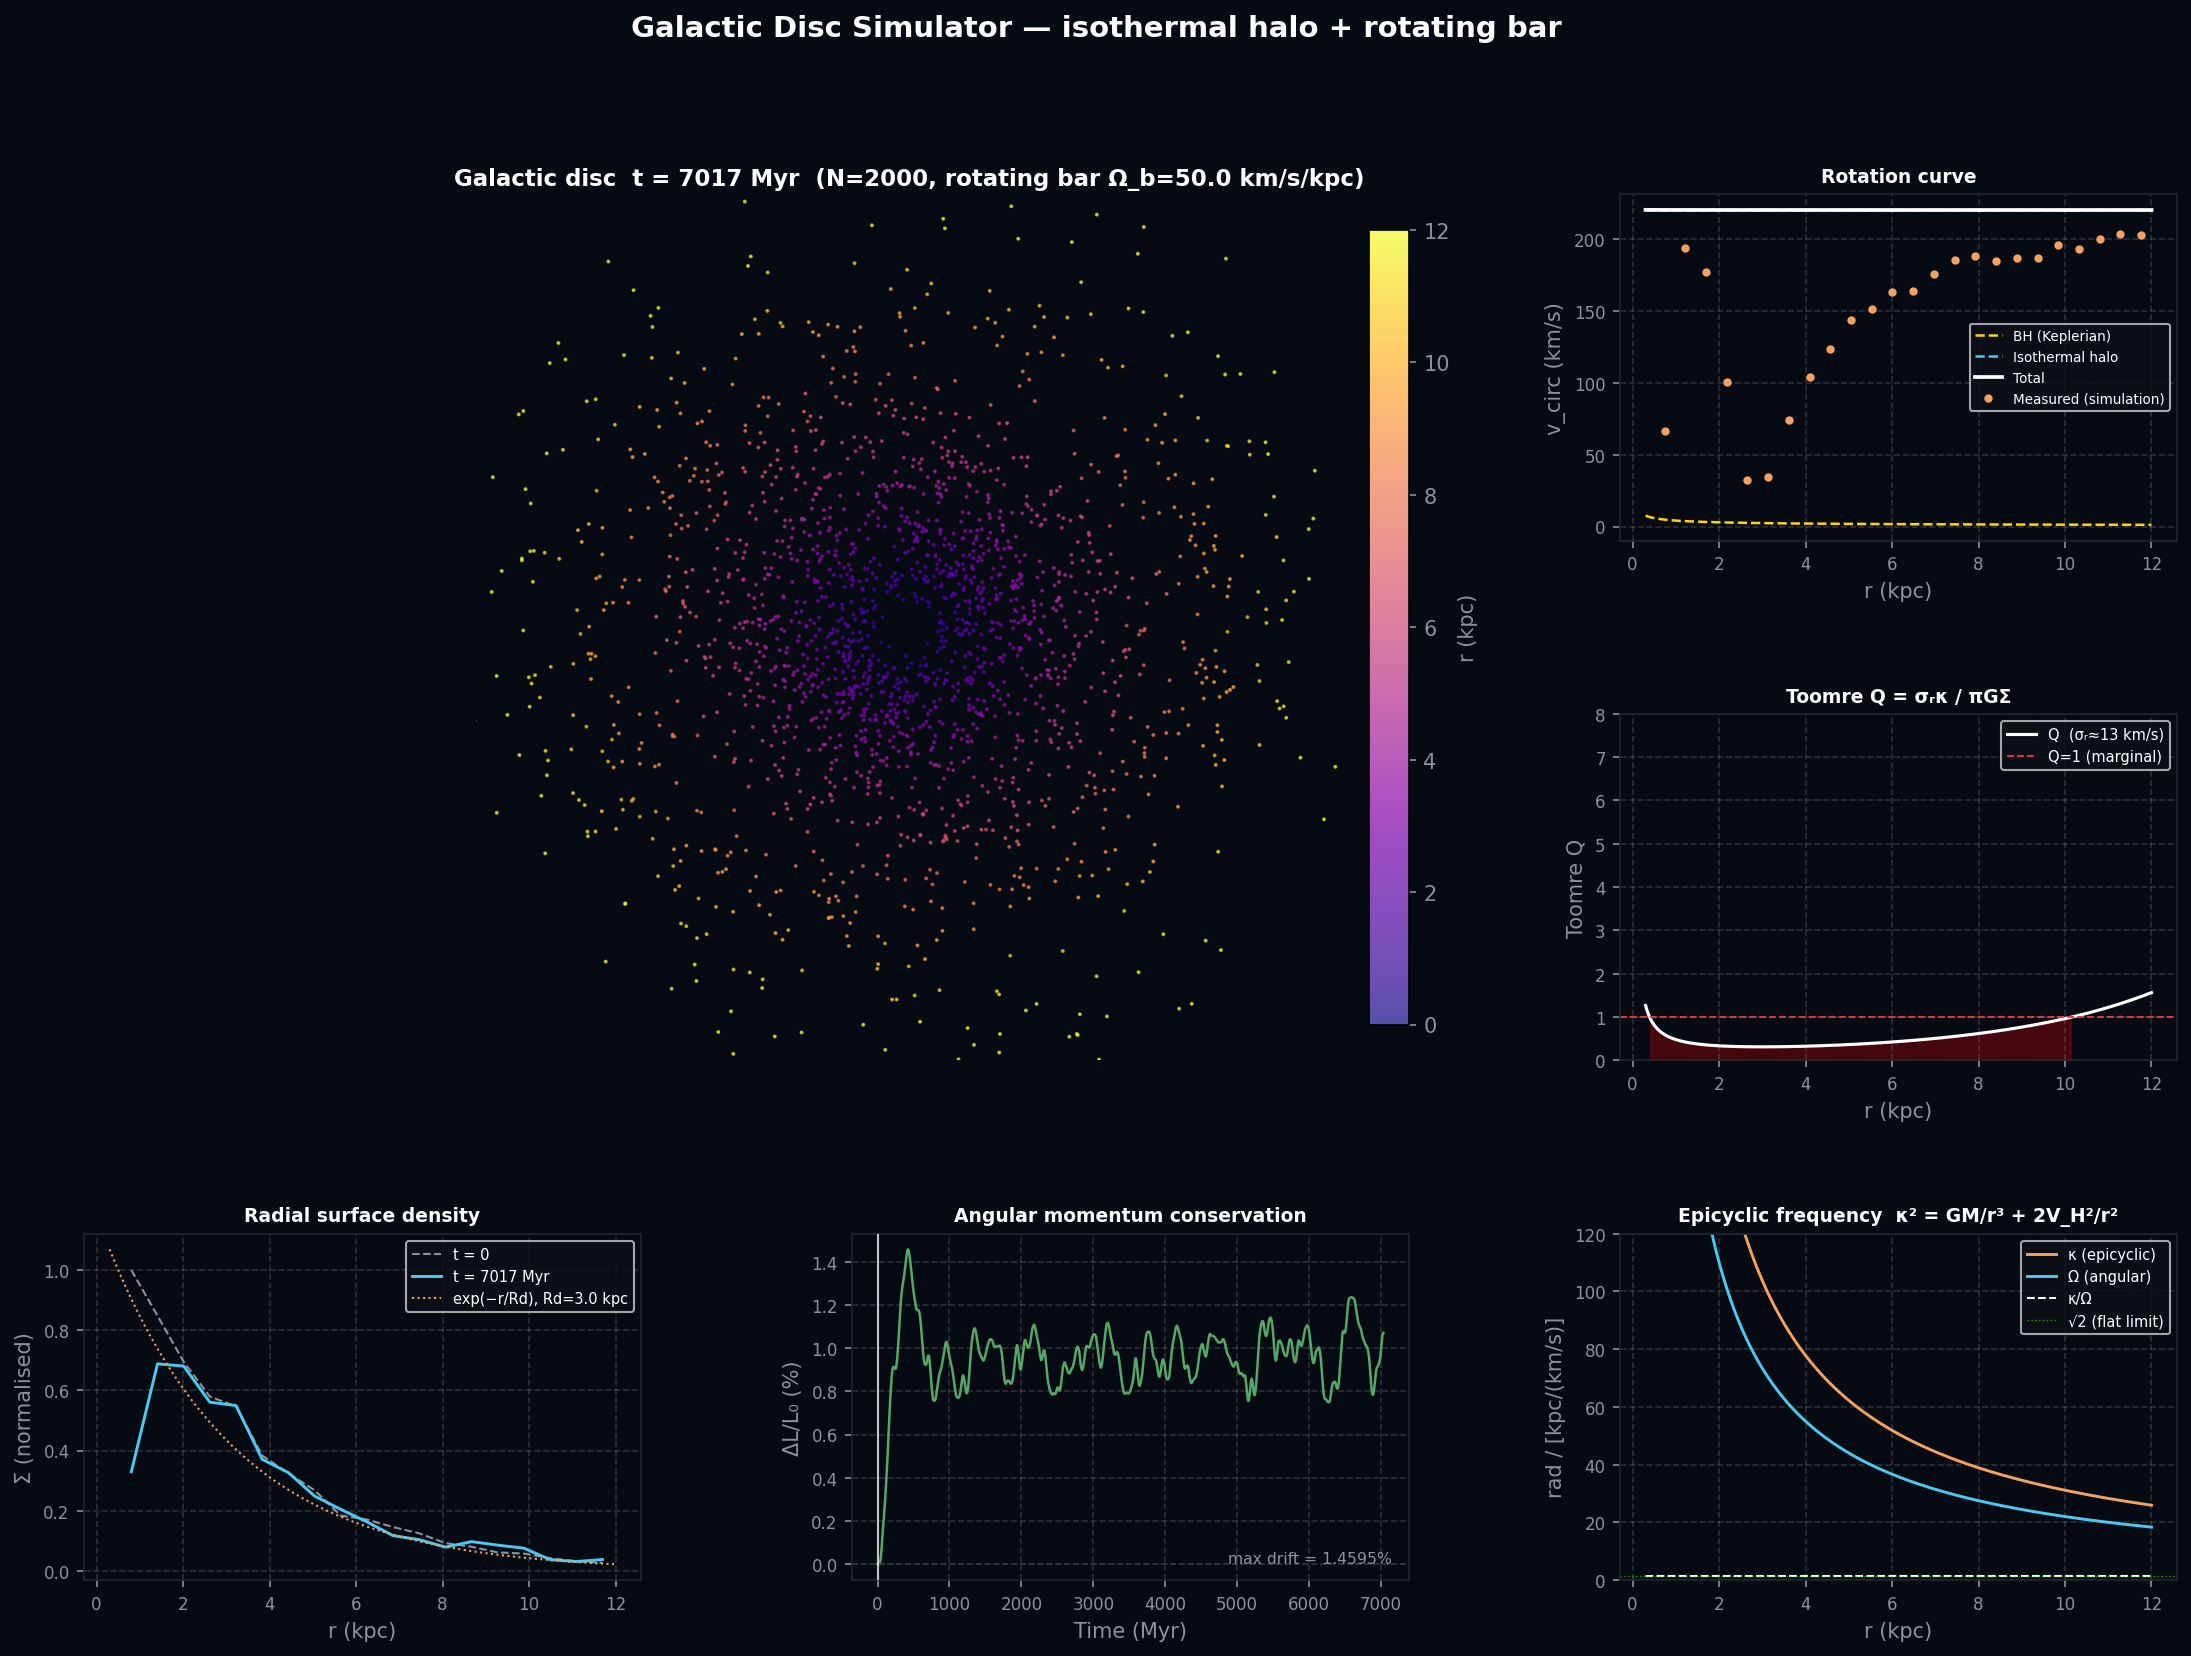
\includegraphics[width=\textwidth]{galaxy_analysis.png}
    \caption{Six-panel analysis output. \textit{Top left:} Final disc snapshot, particles coloured by galactocentric radius. \textit{Top right:} Rotation curve: analytical components (dashed) and total (white), with simulation-measured tangential velocities (orange). \textit{Middle right:} Toomre $Q$ profile; red dashed line marks $Q = 1$. \textit{Bottom left:} Radial surface density at $t=0$ (grey dashed) and $t = 7\,\text{Gyr}$ (blue), normalised to the initial peak. \textit{Bottom middle:} Mean angular momentum drift $\Delta L/L_0$ over the full simulation. \textit{Bottom right:} Epicyclic frequency $\kappa(r)$ and angular frequency $\Omega(r)$, with the flat-curve limit $\kappa/\Omega \to \sqrt{2}$ shown in green.}
    \label{fig:analysis}
\end{figure}

% ─────────────────────────────────────────────────────────────────────────────
\section{Discussion}
\label{sec:discussion}

\subsection{Test-Particle Approximation}

Because particles are massless tracers, the simulation does not capture self-gravity between disc stars. Self-gravity would modify the Toomre stability criterion and amplify spiral density waves, and produce bar slow-down due to dynamical friction from the halo. Future work could incorporate a grid-based Poisson solver (particle-mesh) or direct $O(N^2)$ summation for full self-gravity.

\subsection{Bar Model Limitations}

The bar amplitude $A_\text{bar}$ and pattern speed $\Omega_b$ are held constant throughout the simulation. Real galactic bars slow down as they transfer angular momentum to the halo and disc, and their amplitude evolves with disc mass fraction. A time-varying $\Omega_b(t)$ would produce a more realistic secular evolution, including the outward migration of the corotation resonance.

\subsection{Two-Dimensionality}

The simulation is strictly 2D. Vertical disc structure, bending modes (buckling instability), and the thickening of the bar into a boxy/peanut bulge are not captured. These require a 3D treatment and are significant for comparisons with edge-on galaxies.

% ─────────────────────────────────────────────────────────────────────────────
\section{Conclusion}
\label{sec:conclusion}

We have implemented and validated a test-particle galactic disc simulator incorporating a central black hole, isothermal dark matter halo, and a rotating stellar bar perturbation. The Velocity Verlet integrator conserves angular momentum to within $1.5\%$ over $7\,\text{Gyr}$ and reproduces Keplerian orbits to five significant figures. Key results include: a flat rotation curve at $220\,\text{km\,s}^{-1}$, Toomre-stable disc kinematics ($Q > 1$), bar-driven two-armed spiral structure consistent with corotation at $4.4\,\text{kpc}$, and mild but physically expected angular momentum exchange driven by the non-axisymmetric bar. The code is open-source and available at \url{https://github.com/Harry-670/orbital-simulator}.

% ─────────────────────────────────────────────────────────────────────────────
\bibliographystyle{plainnat}
\begin{thebibliography}{9}

\bibitem[Binney \& Tremaine(2008)]{BinneyTremaine2008}
Binney, J., \& Tremaine, S. (2008).
\newblock \textit{Galactic Dynamics} (2nd ed.).
\newblock Princeton University Press.

\bibitem[Toomre(1964)]{Toomre1964}
Toomre, A. (1964).
\newblock On the gravitational stability of a disk of stars.
\newblock \textit{The Astrophysical Journal}, 139, 1217--1238.

\end{thebibliography}

\end{document}
